\section{Related Work}\label{related}

To take a close look at fault-proneness in object oriented systems, basic object orientation knowledge is important, as explained in section \ref{content}. The paper "\textit{Beyond Language Independent Object-Oriented Metrics: Model Independent Metrics}" \cite{lanza2002beyond} deals not only with the concept of object orientation but also beyond languages and paradigms. The aspects of object orientation such as class, method and attribute can be found as shown in the following tables, which are subdivided into individual metrics. The model from figure \ref{fig0} serves as a template to understand the relationships between the individual metrics. 

In the following tables \ref{tab:classmetrics},\ref{tab:methodmetrics} and \ref{tab:attributesmetrics} the abbrevations and the associated metrics are listed. The used model and the metrics of the tables allow a multiple extension into different research directions. Thus, they fit the principle of object orientation and serve as a basic template to get into the basic structure of metrics. The advantages of this approach are the increased flexibility, i.e., new metamodels can be introduced from any context (for example, the financial world or databases), which provides a standard metric without the need to implement new metrics every time a new context is introduced \cite{lanza2002beyond}. Now, if you look at this system completely from an object orientation perspective, you can see that the basic programming concepts are translated into metrics. Each new method or variable crates more space to generate faults. The complexity of a class is depends, i.e., on the number of methods (NOM) or the number of attributes (NOA), that can be calculated with $NOA = NIV + NCV$, as shown in table \ref{tab:classmetrics}. An important metric about the methods of a class is the number of input parameters (NOP) or the number of access on attributes (NMAA), as you can see in figure \ref{tab:methodmetrics}. For the attribute metrics, the number of direct hits is of great importance, as can be found in figure \ref{tab:attributesmetrics}. 
%Warum sind die Wichtig? Was misst man damit? Coupling? Independence? warum wichtig sagen oder in study xy wird gesagt dass wichtig ist...
%evtl. Tabelle in background weil ist ja zusammenfassung zeug und sowas und darauf baut ja der nächste bums auf

\begin{table}
	\caption{Class metrics from the meta model.}~\label{tab:classmetrics}
	
	\setlength\tabcolsep{3pt}
	\renewcommand{\arraystretch}{1.4}% for the vertical padding
	\begin{tabularx}{\columnwidth}{ | c | p{7cm} | }
		\hline
		Abbrevation & Description \\ \hline\hline
		HNL & Number of classes in superclass chain of class \\ \hline
		NAM & Number of abstract methods \\ \hline
		NCV & Number of class variables \\ \hline
		NIA & Number of inherited attributes \\ \hline
		NIV & Number of instance variables \\ \hline
		NME & Number of methods extended, i.e., redefined in subclass by invoking the same method on a superclass \\ \hline	
		NMI & Number of methods inherited, i.e., defined in superclass and inherited unmodified by subclass\\ \hline
		NMO & Number of methods overridden, i.e., redefined compared to superclass\\ \hline
		NOA & Number of attributes $(NOA = NIV + NCV)$ \\ \hline
		NOC & Number of immediate subclasses of a class \\ \hline
		NOM & Number of methods\\ \hline
		PriA & Number of private attributes (equivalent for protected and public attributes)\\ \hline
		PriM & Number of private methods (equivalent for protected and public attributes)\\ \hline
		SLOC & Sum of all lines of codes over all methods \\ \hline
		WMSG & Sum of message sends in a class\\ \hline
		WNMAA & Number of all accesses on attributes\\ \hline
		WNOC & Number of all descendant classes\\ \hline
		WNOS & Sum of statements in all method bodies of class\\ \hline
		WNI & Number of invocations of all methods \\ \hline
	\end{tabularx}
\end{table}

\begin{table}
	\caption{Method metrics from the meta model.}~\label{tab:methodmetrics}
	
	\setlength\tabcolsep{3pt}
	\renewcommand{\arraystretch}{1.4}% for the vertical padding
	\begin{tabularx}{\columnwidth}{ | c | p{7cm} | }
		\hline
		Abbrevation & Description \\ \hline\hline
		LOC & Method lines of code \\ \hline
		NMA & Number of methods added, i.e., defined in subclass and not in superclass \\ \hline
		MSG & Number of method messages send \\ \hline
		NOP & Number of input parameters \\ \hline
		NI & Number of invocations of other methods within method body \\ \hline
		NMAA & Number of access on attributes \\ \hline
		NOS & Number of statements in method body \\ \hline
	\end{tabularx}
\end{table}

\begin{table}
	\caption{Attribute metrics from the meta model.}~\label{tab:attributesmetrics}
	
	\setlength\tabcolsep{3pt}
	\renewcommand{\arraystretch}{1.4}% for the vertical padding
	\begin{tabularx}{\columnwidth}{ | c | p{7cm} | }
		\hline
		Abbrevation & Description \\ \hline\hline
		AHNL & Class HNL in which attribute is defined \\ \hline
		NAA & Number of times directly accessed \\ \hline
	\end{tabularx}
\end{table}

Many metrics used in various studies are reflected in the tables.
The limitations of this approach are that not all object-oriented software metrics can be defined in terms of the language independent model, but these metrics serve as a basic overview. Certain metrics tend to be very specialized and are therefore difficult to define in a generic way. Another limitation of this basic concept is that for some metrics, there is it is not yet known how best to define them in a generic way, so the meta model does not include coupling metrics and cohesion metrics.

In another paper, a systematic literature review was reviewed that looked at 106 papers published between 1991 and 2011.
Object-oriented metrics (49\%) were used almost twice as often as traditional source code metrics (27\%) or process metrics (24\%). Object-oriented and process-oriented metrics were reported to be more successful in finding bugs compared to traditional size and complexity metrics \cite{b7radjenovic2013software}. The results of the literature review show that an inheritance and an export coupling metric are strongly associated with fault-proneness. Some evidence also suggests that there may be a small number of metrics that are strongly associated with fault-proneness, and that good predictive accuracy and quality estimation accuracy can be achieved with them.

Today's evidence suggests that most faults in software applications are found in a small percentage of software components \cite{b10el2001prediction}. This means that if these faulty software components can be identified early in the lifecycle of the development project, mitigation measures can be taken, such as redesign or refactoring. For object-oriented applications, predictive models using design metrics can be used to identify faulty classes early on \cite{b10el2001prediction}. The next step is to look at related work based on the metrics just presented and expansions of those. 

In the "\textit{Fault-Proneness of Open Source Software: Exploring its Relations to
Internal Software Quality and Maintenance Process}" \cite{kozlov2013fault} study, it was investigated how the fault-proneness of open source software (OSS) can be explained in terms of internal quality attributes and metrics of the maintenance process. A total of 342 releases of these systems were studied and, as usual, software quality was considered as a set of internal and external quality attributes. A total of 76 internal quality attributes were measured and 23 maintenance process metrics were included in this study. The strengths of this study is the comparison of a few software technology trends like fault-proneness and maintainability, as well as the study itself. First the study considers a wide range of metrics than common studies. Furthermore more OOS systems were involved in order to get a better indication of the results. In addition they focused on the fault-proneness of modern Java-based systems and investigated them as an aggregated sample. The framework for assessing the maintenance process was adopted from their previous studies. The results of the factor analysis performed showed that the metrics studied can be interpreted in terms of two factors, one of which is the system size, as shown in Figure \ref{figSize}. Previous studies in this area are based only on relatively small sets of OSS systems and releases, despite the fact that OSS projects are very diverse and heterogeneous \cite{kozlov2013fault}. Conclusively, the results may not be generalizable due to their relatively limited nature. Here, larger systems were chosen and size was found to play an important aspect in fault-proneness. In many other studies only small software systems were considered and it is noticeable that many in their conclusion note that a limitation of their work is that the statements can only be applied to small sized systems \cite{kozlov2013fault, b7radjenovic2013software}.
%evtl eher zu results packen und nicht hier

\begin{figure}[htbp]
	\centerline{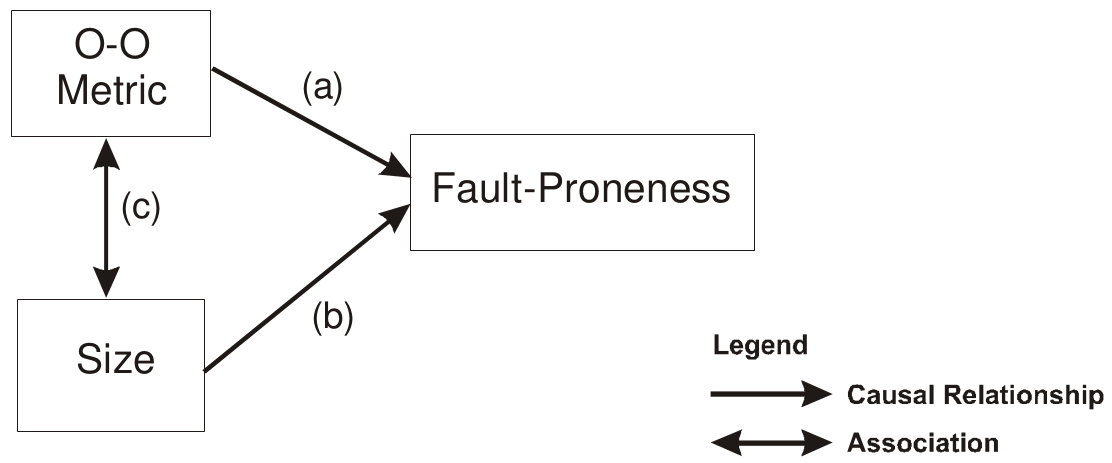
\includegraphics[width=0.45\textwidth]{pictures/faultyclasses2.png}}
	\caption{Path diagram illustrating the confounding effect of class size on the relationship between an object-oriented metric and fault-proneness \cite{b10el2001prediction}.}
	\label{figSize}
\end{figure}

Another study, also dealt with object-oriented design metrics for Java applications and construct a prediction model. It became clear that an export coupling metric exhibited the strongest association with fault-proneness, indicating a structural feature that may be symptomatic of a class with a high probability of latent faults \cite{b10el2001prediction}.

A theoretical basis for developing quantitative models that relate object-oriented metrics and external quality metrics is summarized in Figure \ref{figCoupling}. As already mentioned, one of the strongest association with fault-proneness was an export coupling metric in a study. This illustrates that there is a presumed relationship between object-oriented metrics and fault-proneness due to the effect on cognitive complexity \cite{b10el2001prediction}. Cognitive complexity can be defined as the mental load of the individuals who have to interact with the component, for example, the developers, testers, inspectors, and maintainers. 
%cognitiv complex eher background!

\begin{figure}[htbp]
	\centerline{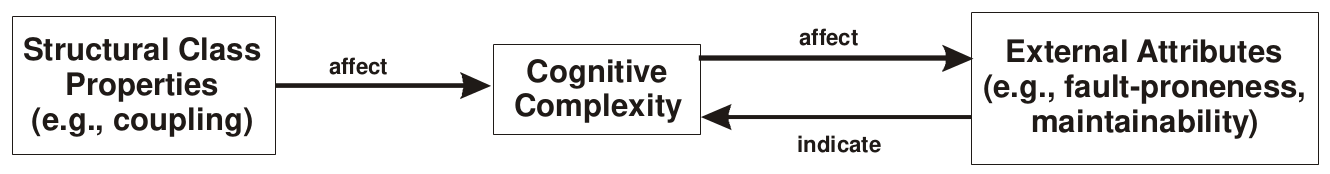
\includegraphics[width=0.5\textwidth]{pictures/faultyclasses1.png}}
	\caption{Theoretical basis for the development of object oriented product metrics \cite{b10el2001prediction}.}
	\label{figCoupling}
\end{figure}

Some studies also suggest that the depth of inheritance has an impact on the comprehensibility of object-oriented applications, and therefore would be expected to have a detrimental effect on fault-proneness \cite{b10el2001prediction}.
It was also found that inheritance leads to distributed class descriptions. That is, in this case, the complete description for a class can only be assembled by examining both the class itself and each of the superclasses of it.
Since different classes are described in different places in the code of a software program, also often distributed over several files, a programmer must turn to several places, in order to receive a complete description of a class. While this argument applies to software source code, it is not difficult to generalize it to design documents. Faults are therefore very distributed and usually cannot be found and fixed in a single place without making other changes.

Another study has considered a used set of ten software product metrics related to the following software attributes: the size of the software, coupling, cohesion, inheritance, and reuse \cite{yu2002predicting}. Some hypotheses regarding fault-proneness were empirically tested in a case study examining the client side of a large network service management system. The system under consideration is written in Java and consists of 123 classes. Validation was performed using two data analysis techniques: regression analysis and discriminant analysis.

Among other things, Class cohesion is a key attribute used to assess the design quality of a class and refers to the extent to which the methods and attributes of a class are related. Typically, classes contain special types of methods, such as constructors, destructors, and access methods, where each of these special methods has its own properties that can affect the measurement of class cohesion \cite{b4al2012impact}. Here we see again that the metrics can all be derived from the tables \ref{tab:classmetrics} and \ref{tab:methodmetrics} below.

Another paper empirically examines this impact of methods on cohesion measures. Twenty existing class cohesion metrics were used and Two types of special methods were considered, constructors and access methods. The empirical study applies the metrics, to five open source systems under four different scenarios, including first considering all special methods, second ignoring only constructors, third ignoring only access methods, and fourth ignoring all special methods.
The results of the empirical investigations show that the cohesion values for most of the considered metrics differ significantly in the four scenarios, but do not significantly affect the abilities of the metrics to predict faulty classes \cite{b4al2012impact}.

Based on this research, two more specific metrics have now been picked out, that try to support the software development process with their metrics. All of them work in their own way and in certain states of development. 
In order to provide guidance on how to proceed in the software process, some special metrics will be explained in detail now.

%Was mache ich/ Was machen andere?
%ABGRENZUNG VON MEINER ARBEIT UND DEREN ARBEIT


%A Validation of Object-Oriented Design Metrics as Quality Indicators ::: his paper presents the results of a study in which we empirically investigated the suite of object-oriented design metrics introduced in. More specifically, our goal is to assess these metrics as predictors of fault-prone classes and, therefore, determine whether they can be used as early quality indicators. This study is complementary to the work described in [30] where the same suite of metrics had been used to assess frequencies of maintenance changes to classes \cite{b11basili1996validation}.



%Assessing the Applicability of Fault-Proneness Models Across Object-Oriented Software Projects ::: Furthermore a number of papers have investigated the relationships between metrics of design and the metrics that detect faults in object oriented software. One of the main objectives of this paper is to assess whether fault-proneness models, based on design measurement, are applicable and can be viable decision making tools when applied from one object-oriented system to the other, in a given environment. \cite{b12riand2002assessing}.



%- kritische auseinandersetzung, für welche fälle sind welche metriken gut und wieso
%- Wann setz ich welche Metriken ein wann im SW Prozess!! und was kann da eintreten passieren
%- Auswirkungen von fehlern
 
%\cite{b7radjenovic2013software}. Context: Software metrics may be used in fault prediction models to improve software quality by predicing fault location. wo wie viele genutzt werden udn so